\section{Results}
\label{sec:results}

\subsection{RQ1: How many and how often do developers delete tests?}

Table \ref{table:deleted-tests-across-version} shows versions selected, total number of days,
total commits, total test deletion commits and total number of deleted tests between the consequtive version
releases.

\begin{table*}[ht!]
    \centering    
    % \aj{A table's caption is above the table, whereas a figure's caption is below the figure}
    \caption{Total numbers of deleted tests and deletion frequency\aj{data is incorrect in the cts and total rows}}
    \label{table:number-of-deleted-test-and-deletion-frequency}
    \begin{tabular}[leftmargin=*]{ |l|c|c|c| }
    \hline
    \thead{Project} & \thead{Num. of test \\deletion commits} & \thead{Num. of \\deleted tests}\\
    \hline
    \makecell{commons-lang} & 107/7,080 (1.5\%) & 866 \\
    \hline
    \makecell{gson} & 39/1,771 (2.2\%) & 260  \\
    \hline
    \makecell{commons-math} & 231/7,116 (3.2\%) & 3,286 \\
    \hline
    \makecell{jfreechart} & 14/4,219 (0.33\%) & 151 \\
    \hline
    \makecell{joda-time} & 31/2,252 (1.38\%) & 662 \\
    \hline
    \makecell{pmd} & 314/25,422 (1.23\%) & 1,826 \\
    \hline
    \makecell{cts} & 1,571/4,710 (0.39\%) & 17,734 \\
    \hline
    \makecell{\textbf{Total}} & \textbf{2,307/401,732 (0.51\%)} & \textbf{24,785} \\
    \hline
    \end{tabular}
    \end{table*}

\begin{table*}[ht!]
    \fontsize{10pt}{10pt}
    \caption{Study of deleted tests across project versions}
    \label{table:deleted-tests-across-version}
    \centering    
    \begin{tabular}{ |l|p{90pt}|p{90pt}|p{90pt}|p{70pt}|p{60pt}| }
    \hline
    \thead{Project} & \thead{Versions} & \thead{Time Period\\(days)} & \thead{Commits}  & \thead{Test Deletion \\ Commits} & \thead{Deleted Tests} \\
    \hline
    \makecell{commons-lang} 
    & \makecell[l]{1.0,2.0,2.1,2.2,2.3,2.4,2.5,\\2.6,3.0,3.1,3.2,3.3,3.4,3.5,\\3.6,3.7,3.8,3.9,3.10,3.11,\\3.12.0}
    & \makecell[l]{1836,0,0,0,0,234,749,284,\\183,119,778,62,397,544,\\196,200,284,\\237,347,111,229}
    & \makecell[l]{155,560,463,357,156,220,\\196,77,1304,236,473,177,\\304,517,315,\\97,147,167,273,242,346 }
    & \makecell[l]{26,0,0,0,0,4,32,5,\\7,3,5,1,1,10,\\4,3,1,1,1,3,0}
    & \makecell[l]{264,0,0,0,0,39,\\374,24,10,30,13,\\6,6,62,9,13,\\1,4,2,9,0 }
    \\
    \hline
    \makecell{gson} 
    & \makecell[l]{1.0,1.1,1.1.1,1.2.2,1.2.3,1.3,\\1.4(beta),1.5,1.6,1.7,1.7.1,\\1.7.2,2.0,2.1,2.2,2.2.1,2.2.2,\\2.2.3,2.2.4,2.3,2.3.1,2.4,2.5,\\2.6,2.6.1,2.6.2,2.7,\\2.8.0,2.8.1,2.8.2,2.8.3,2.8.4,\\2.8.5,2.8.6,2.8.7,2.8.8,2.8.9,\\2.9.0,2.9.1,2.10}
    & \makecell[l]{28,39,17,88,31,\\137,190,314,96,\\138,0,114,99,47,126,5,\\52,283,31,455,\\100,317,51,79,0,14,\\108,134,215,\\112,219,3,20,500,598,\\87,70,104,170,85}
    & \makecell[l]{81,31,6,144,28,107,87,63,\\110,119,8,88,119,88,40,\\7,15,77,13,43,16,\\2110,55,46,4,25,68,\\19,46,21,25,10,12,\\46,46,40,36,45,44,68}
    & \makecell[l]{0,0,0,0,2,2,1,0,\\3,4,0,1,8,5,1,\\0,0,3,0,1,0,0,0,0,0,\\0,0,0,0,0,0,0,0,\\0,0,0,1,2,2,1}
    & \makecell[l]{0,0,0,0,7,5,9,0,\\27,66,0,16,29,53,\\1,0,0,8,0,8,0,0,\\0,0,0,0,0,0,0,0,0,\\0,0,0,0,0,1,25,2,1}
    \\
    \hline
    \makecell{commons-math} 
     & \makecell[l]{1.0,1.1,1.2,2.0,2.1,2.2,3.0,\\3.1,3.2,3.3,3.4,3.5,3.6,\\4.0(beta)}
     & \makecell[l]{1538,0,210,720,45,354,458,\\186,103,403,222,112,\\263,2536}
     & \makecell[l]{696,153,485,771,257,\\393,1680,772,209,549,201,\\80,294,1915}
     & \makecell[l]{37,0,2,21,2,27,18,8,\\2,10,2,12,5,83}
     & \makecell[l]{619,0,7,140,211,\\254,76,22,2,33,6,\\374,12,1522}
     \\
    \hline 
    \makecell{jfreechart} 
    & \makecell[l]{1.0.18,1.0.19,1.5.0,\\1.5.1,1.5.2,1.5.3}
     & \makecell[l]{2561,27,1193,1089,\\62,52 }
     & \makecell[l]{3156,37,428,68,60,42 }
     & \makecell[l]{0,0,8,2,0,0 }
     & \makecell[l]{0,0,126,7,0,0}
     \\ 
    \hline
    \makecell{joda-time} & 
    \makecell[l]{0.9,0.9.5,0.9.8,0.9.9,1.0,1.1,\\1.2,1.2.1,1.3,1.4,1.5,1.5.1,\\1.5.2,1.6.0,1.6.1,1.6.2,\\2.0,2.1,2.2,2.2,2.3,2.4,2.5,\\2.6,2.7,2.8.1,2.8.2,2.9,2.9.1,\\2.9.2,2.9.3,2.9.4,2.9.5,\\2.9.6,2.9.7,2.9.8,2.9.9,\\2.10,2.10.1,2.10.2,2.10.3,\\2.10.4,2.10.5,2.10.6,\\2.10.7,2.10.8,2.10.9,2.10.10,\\2.10.11,2.10.12,2.10.13,\\2.10.14,2.11.0,2.11.1,2.11.2,\\2.12.0,2.12.1,2.12.2,\\2.12.3,2.12.4}
     & \makecell[l]{0,60,264,101,6,169,132,\\52,171,102,350,36,52,\\275,649,36,321,205,\\379,0,161,344,67,59,\\41,154,56,73,19,77,59,\\60,160,7,39,92,0,433,\\150,193,56,77,34,182,\\179,2,66,38,229,6,27,\\144,144,13,31,17,\\16,32,111,0}
      & \makecell[l]{4,143,414,128,12,124,130,\\5,120,54,112,12,9,43,36,6,\\273,35,56,0,49,100,27,15,\\19,35,10,35,4,24,15,8,32,3,\\8,12,2,51,18,20,12,\\8,8,10,10,4,6,4,5,9,4,3,\\13,9,8,17,5,5,13,2}
      & \makecell[l]{0,2,19,0,0,0,2,0,1,0,\\0,0,0,0,3,0,2,0,0,0,0,\\0,0,0,0,0,0,1,0,0,0,\\0,0,0,0,0,0,1,0,0,0,0,0,\\0,0,0,0,0,0,0,0,0,0,\\0,0,0,0,0,0,0}
      & \makecell[l]{0,111,320,0,0,0,18,\\0,1,0,0,0,0,0,161,0,\\46,0,0,0,0,0,0,0,0,\\0,0,2,0,0,0,0,\\0,0,0,0,0,1,0,0,0,\\0,0,0,0,0,0,0,0,0,0,\\0,0,0,0,0,0,0,0,0}
      \\ 
    \hline
    \makecell{pmd} 
    & \makecell[l]{4.3,5.0.0,5.0.1,5.0.2,5.0.3,\\5.0.4,5.0.5,5.1.0,5.1.1,5.1.2,\\5.1.3,5.2.0,5.2.1,5.2.2,5.2.3,\\5.3.0,5.3.1,5.3.2,5.3.3,5.3.4,\\5.3.5,5.3.6,5.3.7,5.3.8,5.4.0,\\5.4.1,5.4.2,5.4.3,5.4.4,5.4.5,\\5.4.6,5.5.0,5.5.1,5.5.2,5.5.3,\\5.5.4,5.5.5,5.5.6,5.5.7,5.7.0,\\5.6.0,5.6.1,5.8.0,5.8.1,6.0.0,\\6.0.1,6.2.0,6.3.0,6.4.0,6.10.0,\\6.11.0,6.12.0,6.13.0,6.14.0,\\6.15.0,6.16.0,6.17.0,6.18.0,\\6.19.0,6.20.0,6.21.0,6.22.0,\\6.23.0,6.24.0,6.25.0,6.26.0,\\6.27.0,6.28.0,6.29.0,6.30.0,\\6.31.0,6.32.0,6.33.0,\\6.34.0,6.35.0,6.36.0,6.37.0,\\6.38.0,6.39.0,6.53.0,6.6.0,\\6.7.0,6.8.0,6.9.0,6.40.0,\\6.41.0,6.42.0,6.43.0,6.44.0,\\6.45.0,6.46.0,6.47.0,6.48.0,\\6.49.0,6.50.0,6.51.0,6.52.0,\\6.53.0,6.54.0,6.55.0,7.0.0}
    & \makecell[l]{3428,172,211,66,61,25,101,\\184,74,84,42,47,16,\\29,17,101,19,31,63,\\54,16,61,148,187,398,\\61,176,159,84,28,\\30,276,32,100,84,28,30,\\22,9,21,29,7,56,6,166,\\37,63,34,30,193,49,\\27,35,27,28,34,27,48,46,\\29,55,47,42,30,33,\\28,37,25,27,48,49,27,28,\\28,34,28,35,27,27,462,\\1617,35,27,28,1097,28,\\62,28,29,33,28,27,35,\\32,29,28,28,35,27,28,28}
    & \makecell[l]{5610,1621,126,30,37,16,17,\\624,48,47,48,74,31,36,26,\\149,15,21,19,39,15,51,89,66,\\329,89,143,85,109,88,55,683,\\57,159,295,159,88,\\8,5,850,94,10,357,19,\\1351,83,370,207,258,1211,\\241,198,175,103,135\\,155,77,174,154,86,210,\\274,299,141,167,194,254,\\78,68,222,151,57,76,88,192,\\110,116,38,48,1424,\\6518,178,118,\\188,4709,98,116,65,148,\\125,123,63,136,63,124,80,\\130,54,124,52,5968}
    & \makecell[l]{138,2,1,1,1,0,0,1,1,0,\\1,1,0,0,0,1,0,1,0,0,0,1,\\1,0,0,1,1,0,3,2,6,0,0,0,\\3,2,6,2,0,0,\\0,0,2,1,6,0,1,0,0,\\4,3,0,1,0,4,1,0,\\5,4,1,11,5,5,5,19,\\0,16,10,5,6,\\8,2,0,0,0,0,1,0,0,26,0,0,\\0,0,116,0,1,4,3,8,1,\\0,3,0,1,0,2,3,0,0,0}
    & \makecell[l]{637,21,20,1,1,0,0,\\2,260,0,16,\\5,0,0,0,1,0,5,0,0,\\0,1,114,0,0,1,\\114,0,3,15,27,0,0,0,\\3,15,27,14,0,0,\\0,0,2,2,12,0,1,0,\\0,7,4,0,1,0,21,\\4,0,95,6,3,64,64,51,\\7,33,0,196,60,\\9,27,31,11,0,0,\\0,0,16,0,0,173\\,0,0,0,0,710,0,2,\\10,108,27,2,\\0,10,0,3,0,8,\\3,0,0,0}
    \\
    \hline
    \makecell{cts} & &  &  &  & \\
    \hline
    \end{tabular}
    \end{table*}



    \begin{figure}[ht!]
        \centering
        \resizebox{\columnwidth}{!}{%
    \begin{tikzpicture}
        \begin{axis}[
            ytick={1,2,3,4,5,6},
            yticklabels={commons-lang, gson, commons-math, jfreechart,joda-time, pmd},
            boxplot/variable width,
            ]
        % commons-lang
        \addplot+ [
        boxplot prepared={
        lower whisker=1, lower quartile=1,
        median=2,
        upper quartile=6.5, upper whisker=140,
        },
        ] coordinates {};
        % gson
        \addplot+ [
        boxplot prepared={
        lower whisker=1, lower quartile=1,
        median=3,
        upper quartile=9, upper whisker=45,
        },
        ] coordinates {};
        % commons-math
        \addplot+ [
        boxplot prepared={
        lower whisker=1, lower quartile=1,
        median=3,
        upper quartile=7, upper whisker=499,
        },
        ] 
        coordinates {};
          % jfreechart
          \addplot+ [
            boxplot prepared={
            lower whisker=1, lower quartile=5,
            median=6,
            upper quartile=8.5, upper whisker=45,
            },
            ] coordinates {};
                % joda-time
          \addplot+ [
            boxplot prepared={
            lower whisker=1, lower quartile=2.5,
            median=6,
            upper quartile=28, upper whisker=137,
            },
            ] coordinates {};
                   % pmd
          \addplot+ [
            boxplot prepared={
            lower whisker=1, lower quartile=1,
            median=2,
            upper quartile=4.5, upper whisker=260,
            },
            ] coordinates {};
        \end{axis}
        \end{tikzpicture}
%
}
\caption{Number of deleted tests in each commit\aj{provide x-axis label}\aj{CTS is missing}}
\end{figure}

\begin{figure}[ht!]
    \centering
    \resizebox{\columnwidth}{!}{%
        \begin{tikzpicture}
            \begin{axis}[
                ytick={1,2,3,4,5,6},
                yticklabels={commons-lang, gson, commons-math, jfreechart,joda-time, pmd},
                boxplot/variable width,
                % width=.8\textwidth,
                % height=.8\textheight,
                ]
            % commons-lang
            \addplot+ [
            boxplot prepared={
            lower whisker=0, lower quartile=1,
            median=22,
            upper quartile=82.25, upper whisker=149,
            },
            ] coordinates {};
            % gson
            \addplot+ [
            boxplot prepared={
            lower whisker=0, lower quartile=3.75,
            median=29,
            upper quartile=104.75, upper whisker=2749,
            },
            ] coordinates {};
            % commons-math
            \addplot+ [
            boxplot prepared={
            lower whisker=0, lower quartile=0,
            median=4.5,
            upper quartile=31, upper whisker=716,
            },
            ] 
            coordinates {};
              % jfreechart
              \addplot+ [
                boxplot prepared={
                lower whisker=0, lower quartile=0,
                median=1,
                upper quartile=114, upper whisker=1093,
                },
                ] coordinates {};
                    % joda-time
              \addplot+ [
                boxplot prepared={
                lower whisker=0, lower quartile=1,
                median=3.5,
                upper quartile=173, upper whisker=1535,
                },
                ] coordinates {};
                       % pmd
              \addplot+ [
                boxplot prepared={
                lower whisker=0, lower quartile=0,
                median=4,
                upper quartile=20, upper whisker=960,
                },
                ] coordinates {};
            \end{axis}
            \end{tikzpicture}
%
}
\caption{Time interval between consecutive test deletion commits\aj{provide x-axis label}\aj{CTS is missing}}
\end{figure}

            \begin{figure}[ht!]
                \centering
                \resizebox{\columnwidth}{!}{%
        \begin{tikzpicture}
            \begin{axis}[
                ytick={1,2,3,4,5,6},
                yticklabels={commons-lang, gson, commons-math, jfreechart,joda-time, pmd},
                boxplot/variable width,
                ]
            % commons-lang
            \addplot+ [
            boxplot prepared={
            lower whisker=1, lower quartile=1,
            median=31.5,
            upper quartile=86.75, upper whisker=441,
            },
            ] coordinates {};
            % gson
            \addplot+ [
            boxplot prepared={
            lower whisker=1, lower quartile=7.75,
            median=19.5,
            upper quartile=45.5, upper whisker=597,
            },
            ] coordinates {};
            % commons-math
            \addplot+ [
            boxplot prepared={
            lower whisker=3, lower quartile=10.45,
            median=40,
            upper quartile=1, upper whisker=303,
            },
            ] 
            coordinates {};
              % jfreechart
              \addplot+ [
                boxplot prepared={
                lower whisker=1, lower quartile=0,
                median=3,
                upper quartile=39, upper whisker=358,
                },
                ] coordinates {};
                    % joda-time
              \addplot+ [
                boxplot prepared={
                lower whisker=1, lower quartile=5,
                median=12,
                upper quartile=61.25, upper whisker=390,
                },
                ] coordinates {};
                       % pmd
              \addplot+ [
                boxplot prepared={
                lower whisker=1, lower quartile=6,
                median=40,
                upper quartile=188.75, upper whisker=5630,
                },
                ] coordinates {};
            \end{axis}
            \end{tikzpicture}
%
}
\caption{Number of commits between consecutive test deletion commits\aj{provide x-axis label}\aj{CTS is missing}}
\end{figure}


\begin{figure}[ht!]
    \centering
    \resizebox{\columnwidth}{!}{%
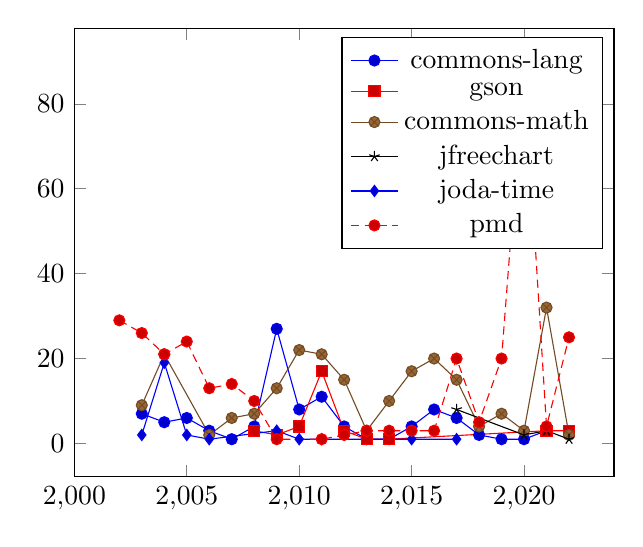
\begin{tikzpicture}
    \begin{axis}
         % commons-lang
    \addplot+ [
        sharp plot,
        ] coordinates {
            (2003,7)
            (2004,5)
            (2005,6)
            (2006,3)
            (2007,1)
            (2008,4)
            (2009,27)
            (2010,8)
            (2011,11)
            (2012,4)
            (2013,1)
            (2014,1)
            (2015,4)
            (2016,8)
            (2017,6)
            (2018,2)
            (2019,1)
            (2020,1)
            (2021,3)
        };
        \addlegendentry{commons-lang}
            % gson
    \addplot+ [
        sharp plot,
        ] coordinates {
            (2008,3)
            (2009,2)
            (2010,4)
            (2011,17)
            (2012,3)
            (2013,1)
            (2014,1)
            (2021,3)
            (2022,3)
        };
        \addlegendentry{gson}
            % commons-math
            \addplot+ [
                sharp plot,
                ] coordinates {
                    (2003,9)
                    (2004,21)
                    (2006,2)
                    (2007,6)
                    (2008,7)
                    (2009,13)
                    (2010,22)
                    (2011,21)
                    (2012,15)
                    (2013,3)
                    (2014,10)
                    (2015,17)
                    (2016,20)
                    (2017,15)
                    (2018,4)
                    (2019,7)
                    (2020,3)
                    (2021,32)
                    (2022,2)
                };
                \addlegendentry{commons-math}
  % jfreechart
  \addplot+ [
    sharp plot,
    ] coordinates {
        (2017,8)
        (2020,2)
        (2021,3)
        (2022,1)
    };
    \addlegendentry{jfreechart}
       % joda-time
       \addplot+ [
        sharp plot,
        ] coordinates {
            (2003,2)
            (2004,19)
            (2005,2)
            (2006,1)
            (2009,3)
            (2010,1)
            (2011,1)
            (2015,1)
            (2017,1)
        };
        \addlegendentry{joda-time}
    % pmd
    \addplot+ [
    sharp plot,
    ] coordinates {
        (2002,29)
        (2003,26)
        (2004,21)
        (2005,24)
        (2006,13)
        (2007,14)
        (2008,10)
        (2009,1)
        (2011,1)
        (2012,2)
        (2013,3)
        (2014,3)
        (2015,3)
        (2016,3)
        (2017,20)
        (2018,5)
        (2019,20)
        (2020,89)
        (2021,4)
        (2022,25)
    };
    \addlegendentry{pmd}
\end{axis}
\end{tikzpicture}
%
}
\caption{Number of test deletion commits\aj{deleted tests, not commits} by year\aj{provide axis labels}\aj{CTS is missing}}
\end{figure}